%%%%%%%%%%%%%%%%%%%%%%%%%%%%%%%%%%%%%%%%%
% Stylish Article
% LaTeX Template
% Version 2.1 (1/10/15)
%
% This template has been downloaded from:
% http://www.LaTeXTemplates.com
%
% Original author:
% Mathias Legrand (legrand.mathias@gmail.com) 
% With extensive modifications by:
% Vel (vel@latextemplates.com)
%
% License:
% CC BY-NC-SA 3.0 (http://creativecommons.org/licenses/by-nc-sa/3.0/)
%
%%%%%%%%%%%%%%%%%%%%%%%%%%%%%%%%%%%%%%%%%

%----------------------------------------------------------------------------------------
%	PACKAGES AND OTHER DOCUMENT CONFIGURATIONS
%----------------------------------------------------------------------------------------

\documentclass[fleqn,10pt]{SelfArx} % Document font size and equations flushed left

\usepackage[english]{babel} % Specify a different language here - english by default

%\usepackage{lipsum} % Required to insert dummy text. To be removed otherwise
%----------------------------------------------------------------------------------------
%	COLUMNS
%----------------------------------------------------------------------------------------

\setlength{\columnsep}{0.55cm} % Distance between the two columns of text
\setlength{\fboxrule}{0.75pt} % Width of the border around the abstract

%----------------------------------------------------------------------------------------
%	COLORS
%----------------------------------------------------------------------------------------

\definecolor{color1}{RGB}{0,0,90} % Color of the article title and sections
\definecolor{color2}{RGB}{0,20,20} % Color of the boxes behind the abstract and headings

%----------------------------------------------------------------------------------------
%	HYPERLINKS
%----------------------------------------------------------------------------------------

\usepackage{hyperref} % Required for hyperlinks
\hypersetup{hidelinks,colorlinks,breaklinks=true,urlcolor=color2,citecolor=color1,linkcolor=color1,bookmarksopen=false,pdftitle={Title},pdfauthor={Author}}

%----------------------------------------------------------------------------------------
%	ARTICLE INFORMATION
%----------------------------------------------------------------------------------------

\JournalInfo{Technical Report 2020-01} % Journal information
\Archive{} % Additional notes (e.g. copyright, DOI, review/research article)

\PaperTitle{Modelling SARS-CoV-2 at Acadia University} % Article title

\Authors{ Duane Currie\textsuperscript{1}, Coleman Hooper\textsuperscript{2}, Margaret Hopkins\textsuperscript{3}, Richard Karsten\textsuperscript{3}, Yifan Li\textsuperscript{4}, Franklin Mendivil\textsuperscript{3}, Holger Teismann\textsuperscript{3}*}
\affiliation{\textsuperscript{1}\textit{Institutional Research, Acadia University, Wolfville, Nova Scotia, Canada}} % Author affiliation
\affiliation{\textsuperscript{2}\textit{????}} % Author affiliation
\affiliation{\textsuperscript{3}\textit{Department of Mathematics and Statistics, Acadia University, Wolfville, Nova Scotia, Canada}} % Author affiliation
\affiliation{\textsuperscript{4}\textit{Jodrey School of Computer Science, Acadia University, Wolfville, Nova Scotia, Canada}} % Author affiliation
\affiliation{*\textbf{Corresponding author}: holger.teismann@acadiau.ca } % Corresponding author


\Keywords{} % Keywords - if you don't want any simply remove all the text between the curly brackets
\newcommand{\keywordname}{Keywords} % Defines the keywords heading name

%----------------------------------------------------------------------------------------
%	ABSTRACT
%----------------------------------------------------------------------------------------

\Abstract{
We are a group consisting of professors, an institutional researcher, and students who are building mathematical and computational models with the goal of informing decisions regarding policies aimed at preventing, detecting and containing a possible outbreak of COVID-19 at Acadia.
Our primary model is based on simulating all of the individuals at Acadia and their interactions.
A strong feature of our effort is the availability of (appropriately anonymized) historical data on class locations, class enrollments, residence room assignments and other similar details of the day-to-day activities of people at Acadia.
This greatly increases the realism of our model and also makes it very specific to the situation at Acadia.\\[5pt]
Using our model we can run simulations of many different combinations of interventions and policy decisions and thereby obtain a quantitative idea of their relative importance in controlling COVID-19.
\emph{We welcome suggestions for combinations with which to experiment. }\\[5pt]
The result of any given simulation run depends on many different random choices since each interaction between an infective individual and a susceptible individual only results in a new infection with a certain probability.
Thus repeating the simulation many times under the same scenario gives statistical information about the range of possible outcomes.\\[5pt]
\emph{We do not claim that the actual numerical values from any simulation are precisely accurate predictions of the progression or final size of an outbreak, only that the relative sizes of the outbreaks under different scenarios are a meaningful comparison of the effects of different combinations of interventions.}\\[5pt]
As an example, we use our model to demonstrate the relative impact of 
different levels of mask-wearing compliance, illustrating that 
high compliance to mask-wearing helps reduce the impact of COVID-19, but not enough to be the only measure used.\\[5pt]
We seek to support the activities of the Fall 2020 Planning Task Force via a collaboration with the task force.
}

\usepackage{xcolor}

\newcommand{\ed}[1]{{\color{blue} #1}}

%----------------------------------------------------------------------------------------

\begin{document}

\flushbottom % Makes all text pages the same height

\maketitle % Print the title and abstract box

\tableofcontents % Print the contents section

\thispagestyle{empty} % Removes page numbering from the first page

%----------------------------------------------------------------------------------------
%	ARTICLE CONTENTS
%----------------------------------------------------------------------------------------

\section{Introduction}

In March when it became clear that Nova Scotia would be significantly impacted by the novel coronavirus pandemic, some of us (R. Karsten and H. Teismann) began investigating the modelling efforts undertaken by colleagues in the Atlantic region. We 
saw a need for epidemiological modelling that would focus on the particular features of our region (such as its demography, 
%(an age structure skewed toward the elderly) and its
rurality, and travel patterns) and on very specific settings such as a residential university in 
a rural town.  We connected with like-minded Atlantic researchers and participated in creating a COVID-19 research network under the auspices of the Atlantic Association for Research in the Mathematical Sciences (AARMS) \href{https://aarms.math.ca/aarms-covid-19-research/}{https://aarms.math.ca/aarms-covid-19-research/}. 


Our local Acadia team includes three professors in Math \& Stats, the Institutional Research Officer, and three undergraduate students.
Our primary task is the construction of a set of models (mathematical and computational) which will allow us to simulate COVID-19 transmission on the Acadia campus.
The goal is to use the models to obtain quantitative evidence of the relative importance of a range of possible interventions and policies aimed at preventing, detecting and controlling a possible outbreak on campus.
For example, is it significantly more effective, in terms of reducing disease spread, to convert all classes with more than 50 people to fully online than it is to divide such large classes into multiple smaller meeting groups in a blended approach?
Our project is similar to a contemporaneous effort for a large university in the United States \cite{gressman2020simulating}, but ours is specifically tailored for the situation at Acadia.

Our primary model is ``agent-based'', which allows modelling of individual-level contact structures and behaviours~\cite{luke_systems_2012,el-sayed_social_2012}.  Using this type of model, we can simulate the interaction of students on campus, and how that relates to transmission of COVID-19.
This includes classes, movement in same buildings between classes, and on-campus residences with more concentrated interaction inside residence sections.  It also allows for simulating the effect of other social interactions.
% DC:  Nothing currently for faculty and staff.  That would be a useful overlay, though.
% For faculty and staff this includes \ed{what....}


We are currently in the testing and validation stage but have some preliminary observations (see below in Section \ref{sec:prelimresults}).



\section{More details on our agent-based model}
An overview of our model is useful in order to be able to understand the types of experiments we are able to perform and also to help interpret any results from these experiments.

Our model begins with a contact network of people, where people are connected if they may regularly be in some degree of contact.  At the beginning, one person at random is marked as infected in a pre-symptomic state, initially exposed to the disease and shortly thereafter becoming infective.  
The simulation of our model advances by moving through time in discrete steps (each such time step could represent one day or a specific portion of a day such as six hours).
During each such step each individual is checked for possible interactions with other individuals according to the contact network given in the model.
Each individual in the model is described as being in one of a possible set of states, be it \emph{susceptible}, \emph{pre-symptomic}, \emph{symptomatic}, \emph{asymptomatic}, \emph{quarantined}, \emph{recovered}, etc.  As the simulation advances and interactions occur, individuals potentially (with some probability) transition from one state to another according to the typical progression of COVID-19.
The transition and transmission probabilities are calibrated so that the disease dynamics generated by our model corresponds to the generally accepted transmission rates and distribution of time periods (latency period, infectious period, serial interval, etc.) for COVID-19.

The possible interactions are governed by a large amount of contact data, which 
is derived from known information about class enrolments, class locations and times, and residence room assignments.
We have built a capability to also include reasonable assumptions about social interaction outside of the academic context, modeled using standard methods from the research literature for simulation of human social contact networks \cite{watts_collective_1998,schnettler_structured_2009,amblard_which_2015}. Because we cannot have precise information about these non-academic interactions, when we include social contact network simulation, we run multiple iterations using repeated sampling of random social contact networks.
Each category of interaction has a certain level of strength, considered in terms of average amount of time in contact, which leads to probabilities of disease transmission that vary with the categories.

\emph{It is important to note that the data being used has been anonymized by subsampling and re-coding of identifiers, and is only available to paid employees of Acadia University.}

The different categories of contact data are encoded separately and thus it is possible to modify each of them independently from the others.
For example, it is simple to remove all classes larger than 50 from the ``classroom contact matrix'' and thus to measure the effect of moving all such classes from face-to-face instruction to fully online instruction.
It is also possible to modify many other aspects of the simulation.
As an example, should Acadia have weekly access to some number of PCR tests for SARS-CoV-2, we could  integrate different testing strategies into the model to determine their expected relative effectiveness %of different randomized testing strategies 
on key measures of interest.  

As an idea, a representative (but incomplete) list of possible experimental factors is:
\begin{enumerate}
    \setlength{\itemsep}{1pt}
    \setlength{\parskip}{0pt}
    \setlength{\parsep}{0pt}

    \item restricting the size of face-to-face classes

    \item splitting single classes into multiple smaller meeting groups

    \item controls on between-class transitions

    \item restricting interaction between residences

    \item partitioning residence sections

    \item cohorting residences by major/program

    \item increased social distancing/mask wearing

    \item testing strategies

    \item contact tracing and quarantine strategies


\end{enumerate}
Of course some of these factors can be more exactly implemented in our model than others, but we are happy to explore a range of possibilities.




\section{Example Application}
\label{sec:prelimresults}


We would describe our simulation model as being in late phases of development.  However, it can already be used to illustrate the impact of some measures to manage the spread of COVID-19.  

As a demonstration of our model, we can examine the effectiveness of masks in reducing the spread of COVID-19.  
Recently, masks were documented as reducing the probability of a respiratory illess spreading between individuals by 44\%  \cite{chu_physical_2020}.  
Using this in a simulation, we can observe the effect of varying degrees of mask-wearing compliance of students.  
In this simulation, we assume class co-enrolment represents 3 hours/week together, passing between classes is of short duration (15 seconds), and average contact between students in the same residence is a few minutes, and between students living in the same residence section is 15 minutes longer on average.  
A recent review of research suggests that 40\%-45\% of cases are asymptomatic, but that university students may be asymptomatic at a higher level \cite{oran_prevalence_2020}.  
In these simulations, we assume cases have a 50\% chance of being asymptomatic.  
For each level of mask compliance, 100 simulations were run with simulated off-campus living situations.  

Figure~\ref{fig:compliance} shows the model's expected number of students infected over time, for mask compliance rates from 0\% up to 100\%.  While there is relatively little impact at low levels of mask compliance, it is clear that a high level of mask compliance (say, 80\% or above) is important to significantly flattening the curve.  It also illustrates two important points regarding mask use:  1) a high degree of mask use helps signficantly; and 2) mask use alone is not enough, and should be combined with other measures.

\begin{figure}[ht]\centering % Using \begin{figure*} makes the figure take up the entire width of the page
	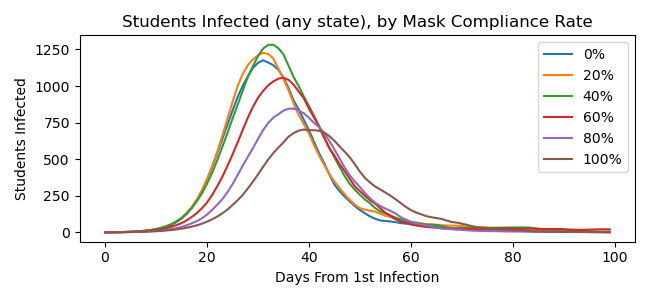
\includegraphics[width=\linewidth]{mask_compliance}
	\caption{Effect of mask compliance on number of students infected within 100 days of first infection on campus.}
	\label{fig:compliance}
\end{figure}

\section{Future plans}

We are currently in the process of reviewing assumptions such as contact durations, social contact network parameters, and distribution of infectivity over time.    Some additional modifications which are being considered relate to integrating additional compliance measures (e.g. case reporting compliance, symptom reporting delays, individual-level mask compliance).
As well, a paper released in pre-print last month for modelling COVID-19 in a large university setting \cite{gressman2020simulating} has also used a fairly similar methodology to ours, and we are reviewing methodological differences to determine if some aspects of their methodology may be appropriate for our model and setting.

After such review, we intend to develop a more extensive technical report outlining in detail our models and results.  While there are some applications of this model that we are currently exploring, we would certainly invite requests from the Planning Committee for questions to explore using our model. 

One area which we have begun exploring is randomized testing strategies.  We have started consulting with statisticians and graph theorists on methods of randomly sampling individuals to test as part of a randomized testing strategy.  In order to evaluate such approaches, we have set up our model to allow us to calculate a variety of measures such as the expected number of individuals infected before a first case is known.

Some research regarding social contact networks of university students suggests that student contact networks are multi-layered and evolve along a combination of social and academic lines \cite{stadtfeld_integration_2019}, and methods that integrate these ideas may improve realism of simulation.

We have been developing our modelling code in such a way as to support public release of the code (but not the data, of course).  
It is structured to help universities simulate disease spread, but with little effort it could be adapted to other similar environments (e.g. colleges, P-12 schools).


\section{Questions for the Fall Planning Task Force}

We are very interested in hearing about the ways that we could help by running ``what-if'' scenarios through our model.
This is true both for planning for the Fall before classes start and also  during the academic year for continued monitoring and any changes which may become necessary as the situation evolves.
To this end:
\begin{itemize}

 \item \emph{ What types of scenarios would be useful to simulate?}

 \item \emph{What operational/policy choices could we try to help clarify?}

 \item \emph{What other aspects might be useful to model?}

\end{itemize}
Feel free to contact any of us.

%------------------------------------------------
\phantomsection
\section*{Acknowledgments} % The \section*{} command stops section numbering
CH, MH, and YL  are funded through NSERC Discovery Grants and Acadia Professional Development funds. 

\addcontentsline{toc}{section}{Acknowledgments} % Adds this section to the table of contents


%----------------------------------------------------------------------------------------
%	REFERENCE LIST
%----------------------------------------------------------------------------------------
\phantomsection
\bibliographystyle{unsrtetal}
\bibliography{references}


%----------------------------------------------------------------------------------------

\end{document}